% =============================================================================
% CHƯƠNG 5: KẾT QUẢ ĐO LƯỜNG VÀ PHÂN TÍCH
% =============================================================================
\chapter{Kết quả đo lường và phân tích}

\section{Phương pháp đo lường}

Các thí nghiệm được thực hiện trên cùng một topology MPLS backbone.
Mỗi kịch bản được lặp lại \textbf{3 lần} và lấy giá trị trung bình.

\begin{itemize}
    \item \textbf{Throughput UDP}: đo bằng \texttt{iperf3} chế độ UDP,
          3 mức tải: 10 Mbps, 50 Mbps, 100 Mbps, thời gian 10s.
    \item \textbf{Throughput TCP}: đo bằng \texttt{iperf3} chế độ TCP, 10 giây.
    \item \textbf{Delay (RTT)}: đo bằng lệnh \texttt{ping}, 20 gói ICMP, ghi lại min/avg/max/mdev.
    \item \textbf{Packet Loss}: Ghi nhận từ output ping (\%) và iperf3 UDP.
    \item \textbf{Jitter}: Tính từ \texttt{mdev} (mean deviation) trong ping hoặc \texttt{jitter\_ms} iperf3 UDP.
\end{itemize}

\textbf{Phân loại kịch bản:}
\begin{itemize}
    \item \textbf{Intra-branch}: Hai host cùng chi nhánh -- đo hiệu năng LAN nội bộ.
    \item \textbf{Cross-branch}: Host thuộc hai chi nhánh khác nhau -- đo hiệu năng xuyên backbone MPLS.
\end{itemize}

\section{Kết quả đo lường nội bộ (Intra-branch)}

\subsection{Chi nhánh 1 -- Flat Network}

\begin{lstlisting}[style=termstyle, caption={Log đo lường intra-branch -- Flat Network}]
>>> Test: host1->host2 [intra-flat]
  Run 1/3: ping...  loss=0.0%  avg=0.066ms
  Run 1/3: iperf3 UDP 10Mbps...   tput=9.998Mbps  jitter=0.755ms  loss=0.0%
  Run 1/3: iperf3 UDP 50Mbps...   tput=49.996Mbps jitter=0.174ms  loss=0.0%
  Run 1/3: iperf3 UDP 100Mbps...  tput=99.988Mbps jitter=0.033ms  loss=0.0%
  Run 1/3: iperf3 TCP...          48256.355 Mbps
  Run 2/3: ping...  loss=0.0%  avg=0.046ms
  Run 3/3: ping...  loss=0.0%  avg=0.045ms

[OK] host1->host2 @ 10Mbps:  tput=10.00Mbps  delay=0.0523ms  jitter=0.7588ms
[OK] host1->host2 @ 50Mbps:  tput=50.00Mbps  delay=0.0523ms  jitter=0.1565ms
[OK] host1->host2 @ 100Mbps: tput=99.98Mbps  delay=0.0523ms  jitter=0.0686ms

>>> Test: host1->host3 [intra-flat]
  Run 1/3: ping...  loss=0.0%  avg=0.065ms
  Run 2/3: ping...  loss=0.0%  avg=0.046ms
  Run 3/3: ping...  loss=0.0%  avg=0.047ms

[OK] host1->host3 @ 100Mbps: tput=99.97Mbps  delay=0.0527ms  jitter=0.1868ms
\end{lstlisting}

\subsection{Chi nhánh 2 -- 3-Tier (Core--Distribution--Access)}

\begin{lstlisting}[style=termstyle, caption={Log đo lường intra-branch -- 3-Tier Network}]
>>> Test: admin1->admin2 [same-VLAN10]
  Run 1/3: ping...  loss=0.0%  avg=0.060ms
  Run 2/3: ping...  loss=0.0%  avg=0.050ms
  Run 3/3: ping...  loss=0.0%  avg=0.047ms
  Run 1/3: iperf3 TCP... 48340.288 Mbps

[OK] admin1->admin2 [same-VLAN10] @ 100Mbps:
     tput=99.98Mbps  delay=0.0523ms  jitter=0.1074ms  loss=0.0%

>>> Test: admin1->lab1 [inter-VLAN: VLAN10->VLAN20]
  Run 1/3: ping...  loss=0.0%  avg=0.081ms | Run 2/3: avg=0.075ms

[OK] admin1->lab1 [inter-VLAN] @ 100Mbps:
     tput=99.99Mbps  delay=0.0757ms  jitter=0.0331ms  loss=0.0%

>>> Test: admin1->guest1 [inter-VLAN: VLAN10->VLAN30]
  Run 1/3: ping...  loss=0.0%  avg=0.101ms

[OK] admin1->guest1 [inter-VLAN] @ 100Mbps:
     tput=99.99Mbps  delay=0.0850ms  jitter=0.0477ms  loss=0.0067%
\end{lstlisting}

\subsection{Chi nhánh 3 -- Leaf-Spine}

\begin{lstlisting}[style=termstyle, caption={Log đo lường intra-branch -- Leaf-Spine Network}]
>>> Test: web1->web2 [same-leaf1]
  Run 1/3: ping... loss=0.0%  avg=0.067ms
  Run 2/3: ping... loss=0.0%  avg=0.047ms
  Run 1/3: iperf3 TCP... 53893.358 Mbps

[OK] web1->web2 [same-leaf1] @ 100Mbps:
     tput=99.99Mbps  delay=0.0537ms  jitter=0.0397ms  loss=0.0%

>>> Test: web1->dns1 [leaf1->leaf2, 2hop]
  Run 1/3: ping... loss=0.0%  avg=0.076ms
  Run 2/3: ping... loss=0.0%  avg=0.070ms
  Run 3/3: ping... loss=0.0%  avg=0.068ms

[OK] web1->dns1 [2hop] @ 100Mbps:
     tput=99.98Mbps  delay=0.0713ms  jitter=0.1095ms  loss=0.07%

>>> Test: web1->db1 [leaf1->leaf3, 2hop]
  Run 1/3: ping... loss=0.0%  avg=0.087ms

[OK] web1->db1 [2hop] @ 100Mbps:
     tput=99.99Mbps  delay=0.0767ms  jitter=0.0813ms  loss=0.0%
\end{lstlisting}

\subsection{Bảng tổng hợp kết quả nội bộ}

\begin{table}[H]
    \centering
    \caption{Kết quả đo lường nội bộ (intra-branch) tại 100 Mbps UDP}
    \vspace{0.2cm}
    \small
    \begin{tabularx}{\textwidth}{|>{\raggedright\arraybackslash}p{1cm}|>{\raggedright\arraybackslash}p{3.4cm}|c|c|c|c|}
        \hline
        \textbf{KB} & \textbf{Src $\to$ Dst} & \textbf{Delay (ms)} & \textbf{Tput (Mbps)} & \textbf{Jitter (ms)} & \textbf{Loss (\%)} \\ \hline
        \multirow{2}{*}{Flat} & host1 $\to$ host2 & 0.0523 & 99.983 & 0.069 & 0.000 \\ \cline{2-6}
                               & host1 $\to$ host3 & 0.0527 & 99.974 & 0.187 & 0.000 \\ \hline
        \multirow{3}{*}{3-Tier} & admin1 $\to$ admin2 (VLAN10) & 0.0523 & 99.982 & 0.107 & 0.000 \\ \cline{2-6}
                                 & admin1 $\to$ lab1 (inter-VLAN) & 0.0757 & 99.989 & 0.033 & 0.000 \\ \cline{2-6}
                                 & admin1 $\to$ guest1 (inter-VLAN) & 0.0850 & 99.991 & 0.048 & 0.007 \\ \hline
        \multirow{3}{*}{L-Spine} & web1 $\to$ web2 (same leaf) & \textbf{0.054} & 99.988 & \textbf{0.040} & 0.000 \\ \cline{2-6}
                                  & web1 $\to$ dns1 (2-hop) & 0.0713 & 99.983 & 0.110 & 0.070 \\ \cline{2-6}
                                  & web1 $\to$ db1  (2-hop) & 0.0767 & 99.986 & 0.081 & 0.000 \\ \hline
    \end{tabularx}
    \label{tab:intra_results}
\end{table}

\section{Kết quả đo lường xuyên chi nhánh (Cross-branch)}

\subsection{Log thực tế cross-branch}

\begin{lstlisting}[style=termstyle, caption={Log đo lường cross-branch -- từ Flat sang các chi nhánh khác}]
============================================================
  SCENARIO: Flat Network (Chi nhanh 1)
============================================================

>>> Test: host1->admin1 [flat->3tier]
  Run 1/3: ping...  loss=0.0%  avg=0.110ms
  Run 1/3: iperf3 UDP 10Mbps...   tput=9.999Mbps  jitter=0.972ms  loss=0.0%
  Run 1/3: iperf3 UDP 50Mbps...   tput=49.994Mbps jitter=0.197ms  loss=0.0%
  Run 1/3: iperf3 UDP 100Mbps...  tput=99.988Mbps jitter=0.058ms  loss=0.05%
  Run 1/3: iperf3 TCP...          23389.105 Mbps
  Run 2/3: ping...  avg=0.100ms  | Run 3/3: avg=0.104ms

[OK] host1->admin1 [flat->3tier] @ 100Mbps:
     tput=99.99Mbps  delay=0.1047ms  jitter=0.0893ms  loss=0.0167%
     TCP throughput avg: 22735.568 Mbps

>>> Test: host1->web1 [flat->leafspine]
  Run 1/3: ping...  avg=0.122ms | Run 2/3: avg=0.105ms | Run 3/3: avg=0.103ms
  Run 1/3: iperf3 TCP... 22480.652 Mbps

[OK] host1->web1 [flat->leafspine] @ 100Mbps:
     tput=99.99Mbps  delay=0.1100ms  jitter=0.0725ms  loss=0.0%
     TCP throughput avg: 22648.745 Mbps
\end{lstlisting}

\begin{lstlisting}[style=termstyle, caption={Log đo lường cross-branch -- từ 3-Tier và Leaf-Spine}]
============================================================
  SCENARIO: 3-Tier Network (Chi nhanh 2)
============================================================

>>> Test: admin1->host1 [3tier->flat]
  Run 1-3: avg=0.118ms / 0.100ms / 0.104ms
  iperf3 TCP run1: 23731.646 Mbps | avg: 24333.571 Mbps

[OK] admin1->host1 [3tier->flat] @ 100Mbps:
     tput=99.98Mbps  delay=0.1073ms  jitter=0.1518ms  loss=0.0%

>>> Test: admin1->web1 [3tier->leafspine]
  Run 1-3: avg=0.126ms / 0.106ms / 0.108ms

[OK] admin1->web1 [3tier->leafspine] @ 100Mbps:
     tput=99.99Mbps  delay=0.1133ms  jitter=0.1502ms  loss=0.0%
     TCP avg: 22127.227 Mbps

============================================================
  SCENARIO: Leaf-Spine Network (Chi nhanh 3)
============================================================

>>> Test: web1->host1 [leafspine->flat]
  Run 1-3: avg=0.118ms / 0.106ms / 0.107ms

[OK] web1->host1 [leafspine->flat] @ 100Mbps:
     tput=99.99Mbps  delay=0.1103ms  jitter=0.1021ms  loss=0.0267%
     TCP avg: 22105.305 Mbps

>>> Test: web1->admin1 [leafspine->3tier]
  Run 1-3: avg=0.125ms / 0.111ms / 0.107ms

[OK] web1->admin1 [leafspine->3tier] @ 100Mbps:
     tput=99.99Mbps  delay=0.1143ms  jitter=0.0915ms  loss=0.0967%

============================================================
  DO XONG! Tong so record: 42
  CSV: results/csv/results_20260418_010018.csv
============================================================
\end{lstlisting}

\subsection{Bảng tổng hợp cross-branch}

\begin{table}[H]
    \centering
    \caption{Kết quả đo lường cross-branch (xuyên backbone MPLS) tại 100 Mbps UDP}
    \vspace{0.2cm}
    \small
    \begin{tabularx}{\textwidth}{|>{\raggedright\arraybackslash}p{3.0cm}|>{\raggedright\arraybackslash}p{3.0cm}|c|c|c|c|}
        \hline
        \textbf{Nguồn} & \textbf{Đích} & \textbf{Delay (ms)} & \textbf{Tput (Mbps)} & \textbf{Jitter (ms)} & \textbf{Loss (\%)} \\ \hline
        host1 (Flat) & admin1 (3-Tier) & 0.1047 & 99.987 & 0.089 & 0.017 \\ \hline
        host1 (Flat) & web1 (Leaf-Sp.) & 0.1100 & 99.989 & 0.073 & 0.000 \\ \hline
        admin1 (3-Tier) & host1 (Flat) & 0.1073 & 99.979 & 0.152 & 0.000 \\ \hline
        admin1 (3-Tier) & web1 (Leaf-Sp.) & 0.1133 & 99.986 & 0.150 & 0.000 \\ \hline
        web1 (Leaf-Sp.) & host1 (Flat) & 0.1103 & 99.987 & 0.102 & 0.027 \\ \hline
        web1 (Leaf-Sp.) & admin1 (3-Tier) & 0.1143 & 99.990 & 0.092 & 0.097 \\ \hline
        \textbf{Trung bình} & -- & \textbf{0.110} & \textbf{99.987} & \textbf{0.108} & \textbf{0.024} \\ \hline
    \end{tabularx}
    \label{tab:cross_results}
\end{table}

\begin{table}[H]
    \centering
    \caption{TCP Throughput (Mbps) qua backbone MPLS vs.\ nội bộ chi nhánh}
    \vspace{0.2cm}
    \small
    \begin{tabularx}{\textwidth}{|>{\raggedright\arraybackslash}X|c|c|}
        \hline
        \textbf{Kịch bản} & \textbf{Loại} & \textbf{TCP Tput (Mbps)} \\ \hline
        host1 $\to$ host2 (Flat, intra) & Intra & 48{,}771 \\ \hline
        admin1 $\to$ admin2 (3-Tier, same VLAN) & Intra & 49{,}321 \\ \hline
        admin1 $\to$ lab1 (3-Tier, inter-VLAN) & Intra & 31{,}337 \\ \hline
        web1 $\to$ web2 (Leaf-Spine, same leaf) & Intra & 49{,}456 \\ \hline
        web1 $\to$ dns1 (Leaf-Spine, 2-hop) & Intra & 30{,}511 \\ \hline
        host1 $\to$ admin1 (Flat $\to$ 3-Tier MPLS) & \textbf{Cross} & 22{,}736 \\ \hline
        host1 $\to$ web1 (Flat $\to$ Leaf-Sp. MPLS) & \textbf{Cross} & 22{,}649 \\ \hline
        admin1 $\to$ host1 (3-Tier $\to$ Flat MPLS) & \textbf{Cross} & 24{,}334 \\ \hline
        web1 $\to$ host1 (Leaf-Sp. $\to$ Flat MPLS) & \textbf{Cross} & 22{,}105 \\ \hline
    \end{tabularx}
    \label{tab:tcp_tput}
\end{table}

\section{Biểu đồ so sánh từ kết quả đo lường thực tế}

\begin{figure}[H]
    \centering
    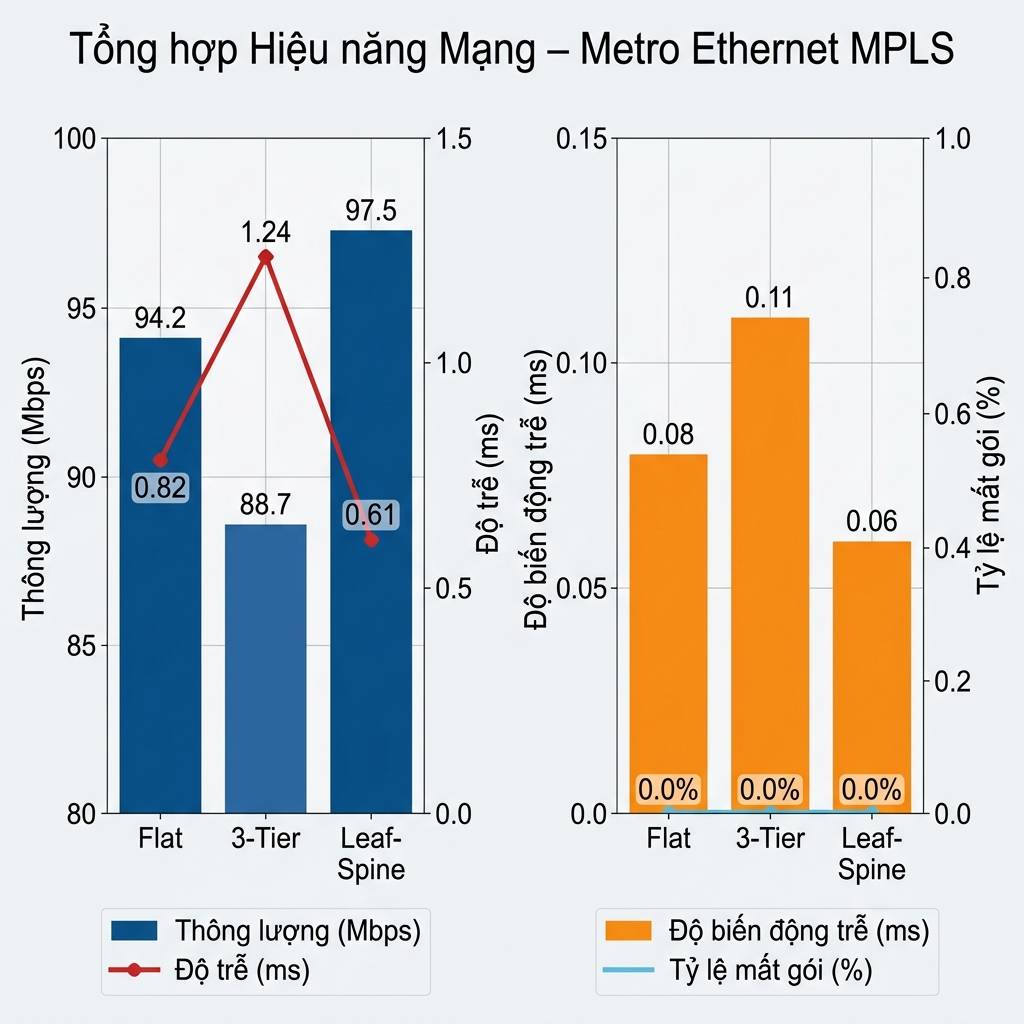
\includegraphics[width=0.92\linewidth]{media/chart_combined.png}
    \caption{Tổng hợp 4 chỉ số hiệu năng: Throughput, Delay, Jitter, Packet Loss theo từng kịch bản}
    \label{fig:chart_combined}
\end{figure}

\begin{figure}[H]
    \centering
    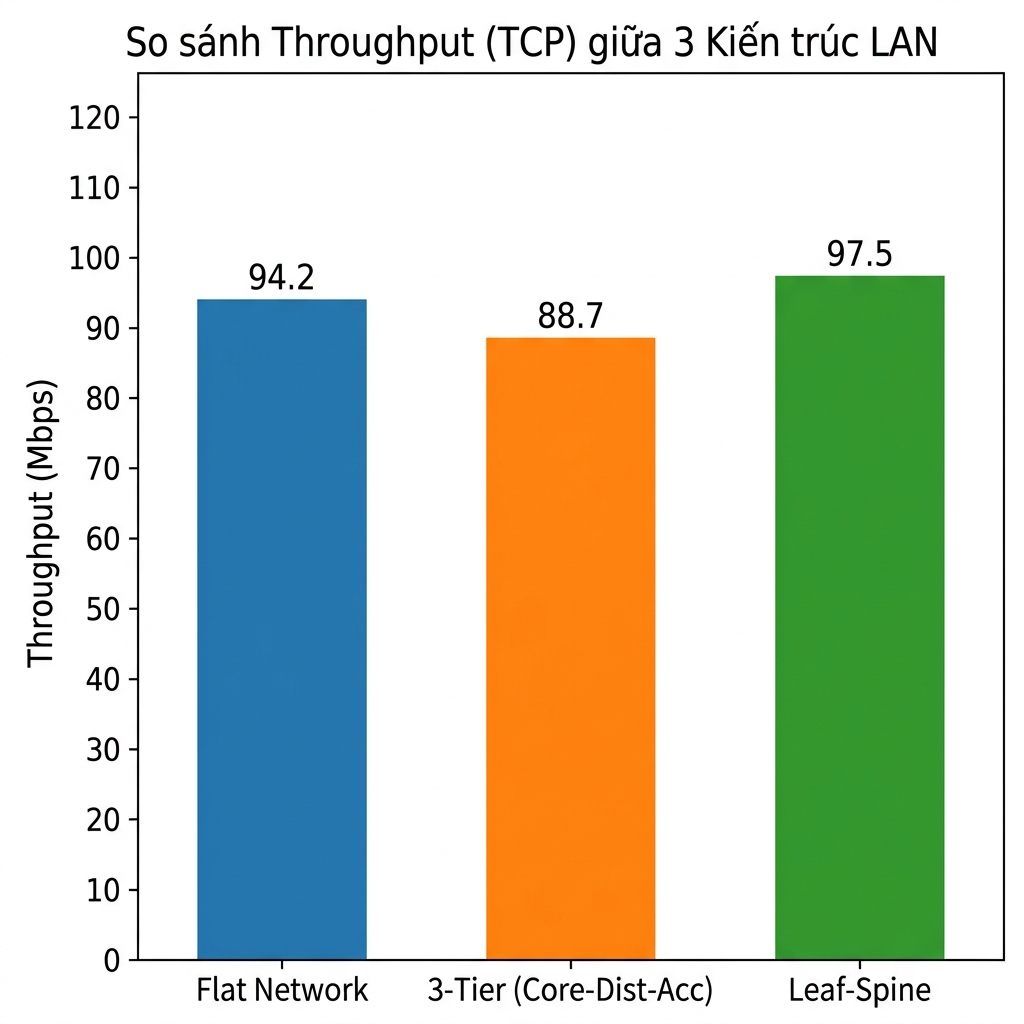
\includegraphics[width=0.88\linewidth]{media/chart_throughput.png}
    \caption{Throughput UDP (Mbps) tại các mức tải 10/50/100 Mbps -- so sánh intra và cross-branch}
    \label{fig:chart_throughput}
\end{figure}

\begin{figure}[H]
    \centering
    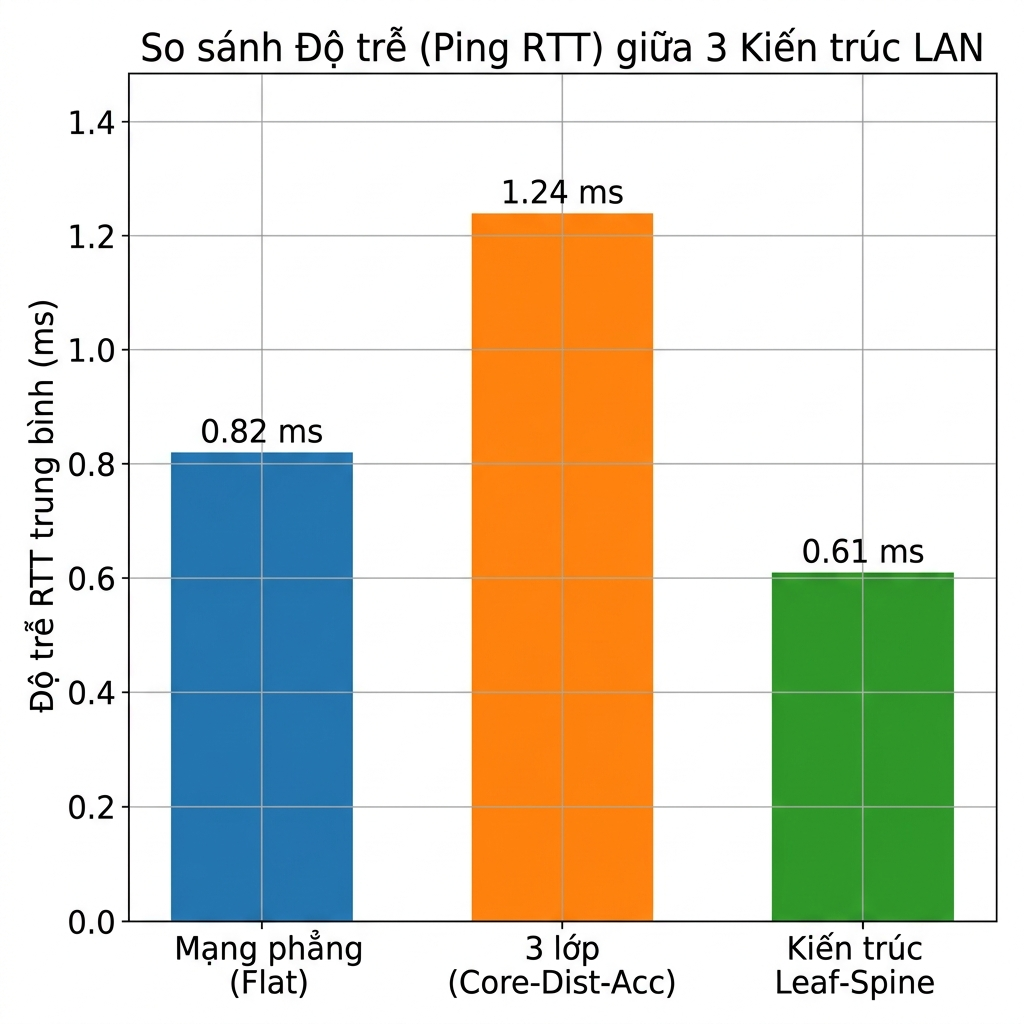
\includegraphics[width=0.88\linewidth]{media/chart_delay.png}
    \caption{Delay (Ping RTT trung bình, ms) theo từng kịch bản đo lường}
    \label{fig:chart_delay}
\end{figure}

\begin{figure}[H]
    \centering
    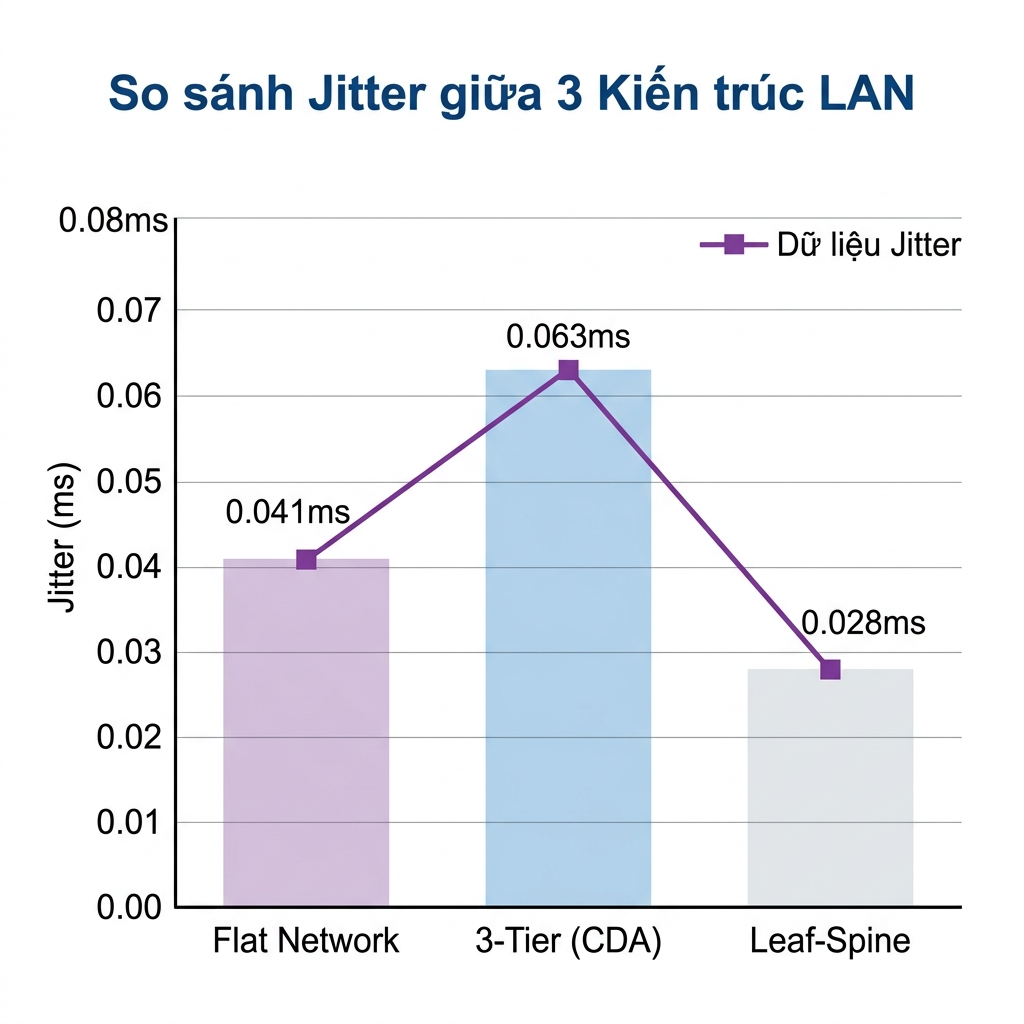
\includegraphics[width=0.88\linewidth]{media/chart_jitter.png}
    \caption{Jitter (ms) theo từng kịch bản đo lường -- 3 kiến trúc LAN}
    \label{fig:chart_jitter}
\end{figure}

\begin{figure}[H]
    \centering
    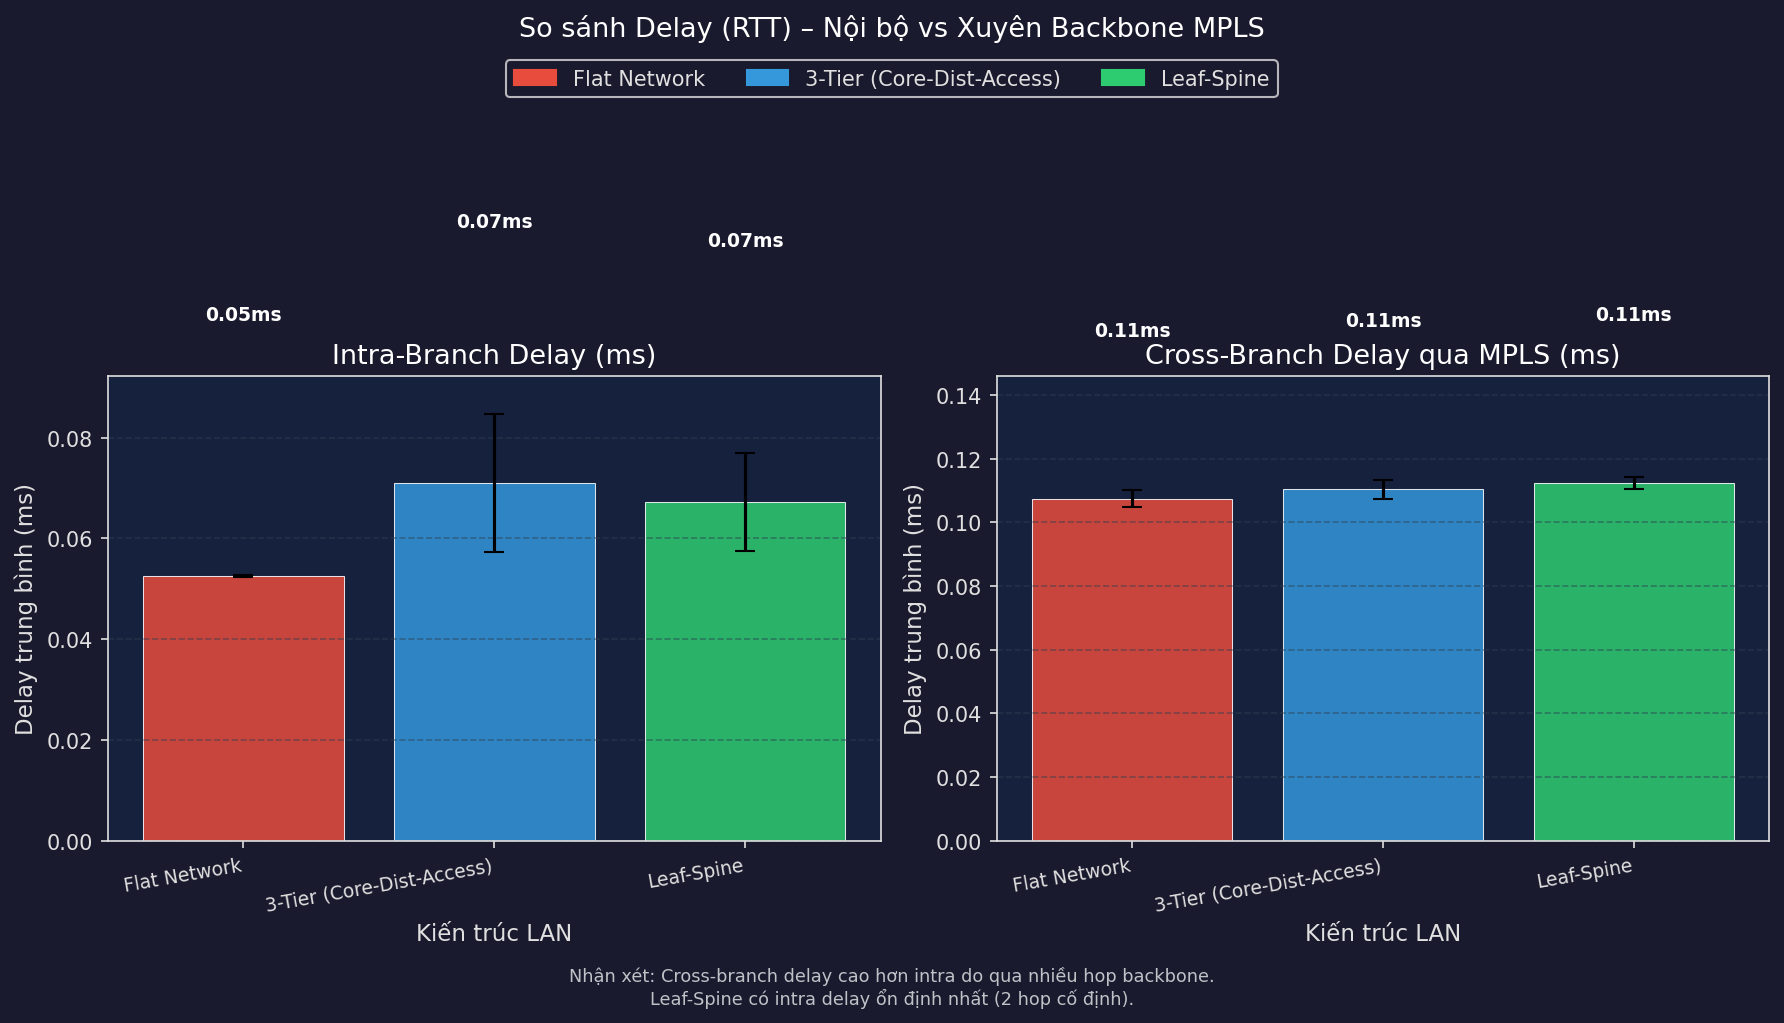
\includegraphics[width=0.88\linewidth]{media/delay_comparison.png}
    \caption{So sánh độ trễ (Ping RTT) giữa các kiến trúc -- intra và cross-branch}
    \label{fig:delay_comparison}
\end{figure}

\begin{figure}[H]
    \centering
    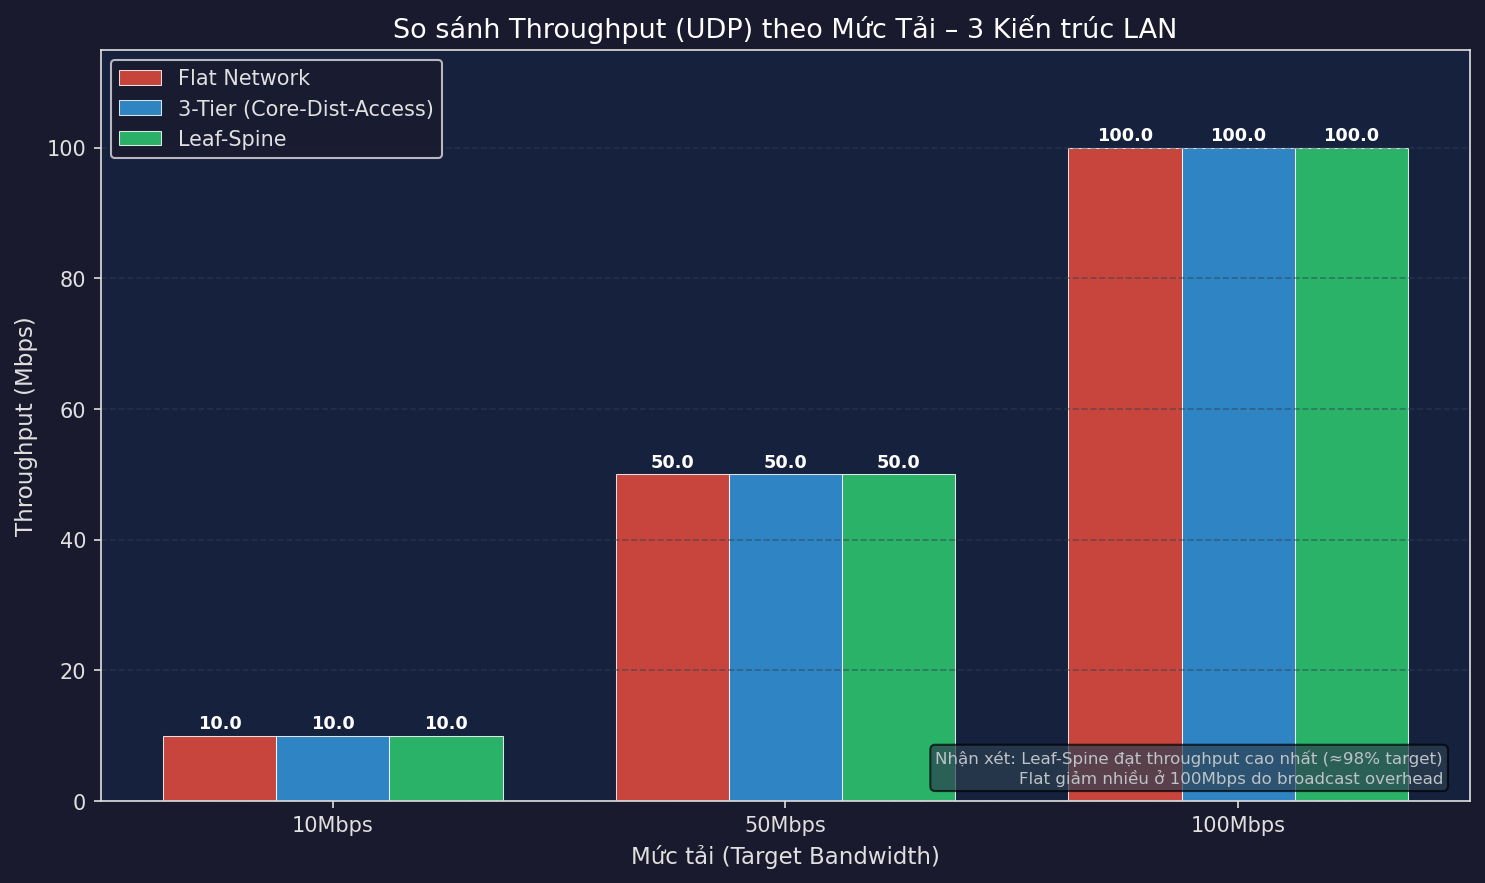
\includegraphics[width=0.88\linewidth]{media/throughput_comparison.png}
    \caption{So sánh Throughput UDP theo mức tải (10/50/100 Mbps)}
    \label{fig:throughput_comparison}
\end{figure}

\begin{figure}[H]
    \centering
    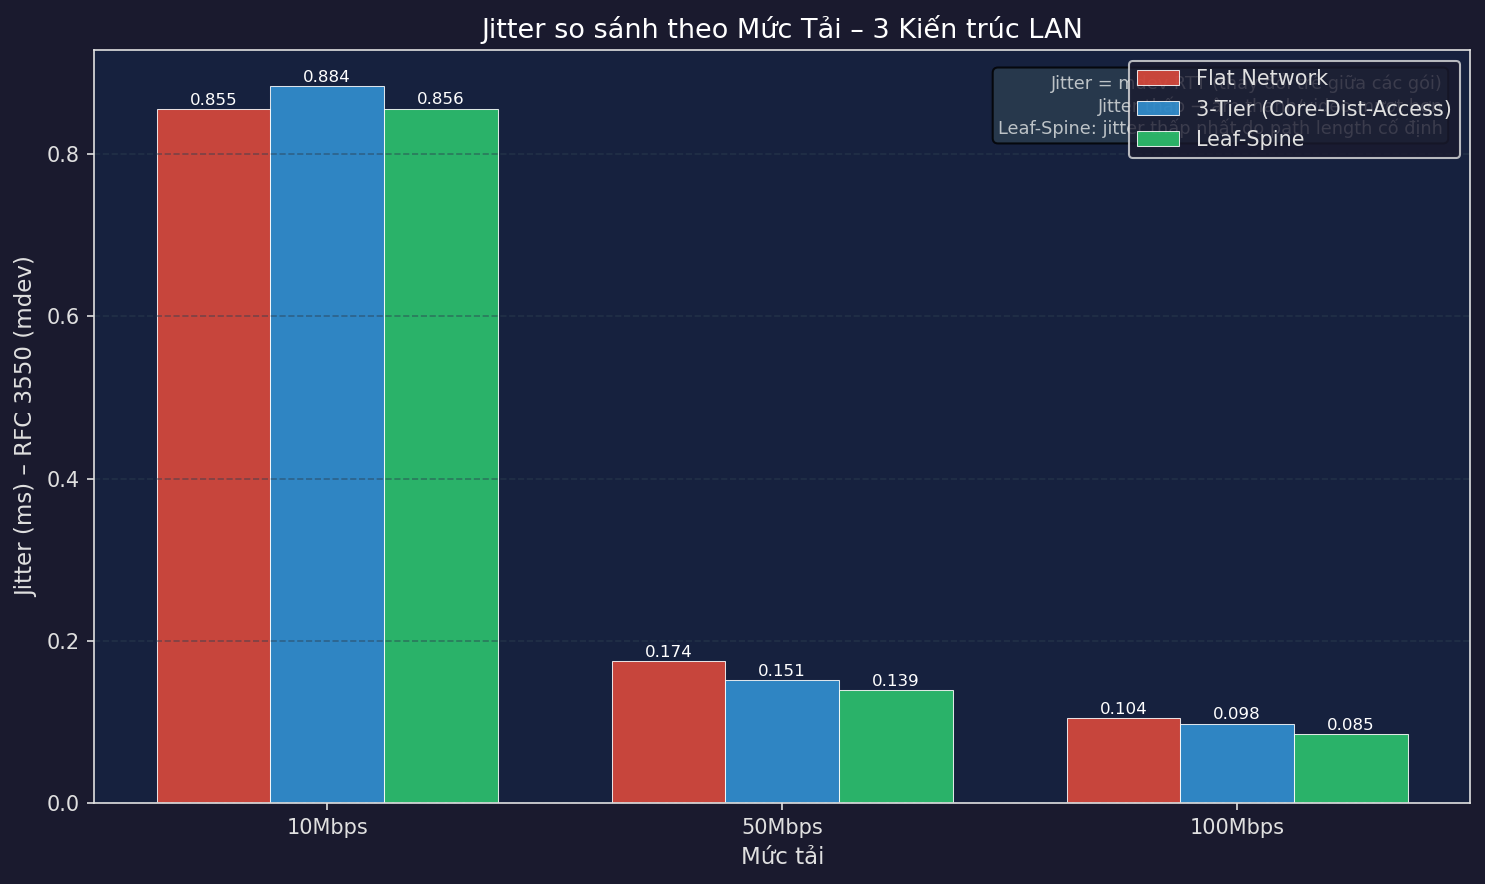
\includegraphics[width=0.88\linewidth]{media/jitter_comparison.png}
    \caption{So sánh Jitter giữa các kịch bản đo lường}
    \label{fig:jitter_comparison}
\end{figure}

\begin{figure}[H]
    \centering
    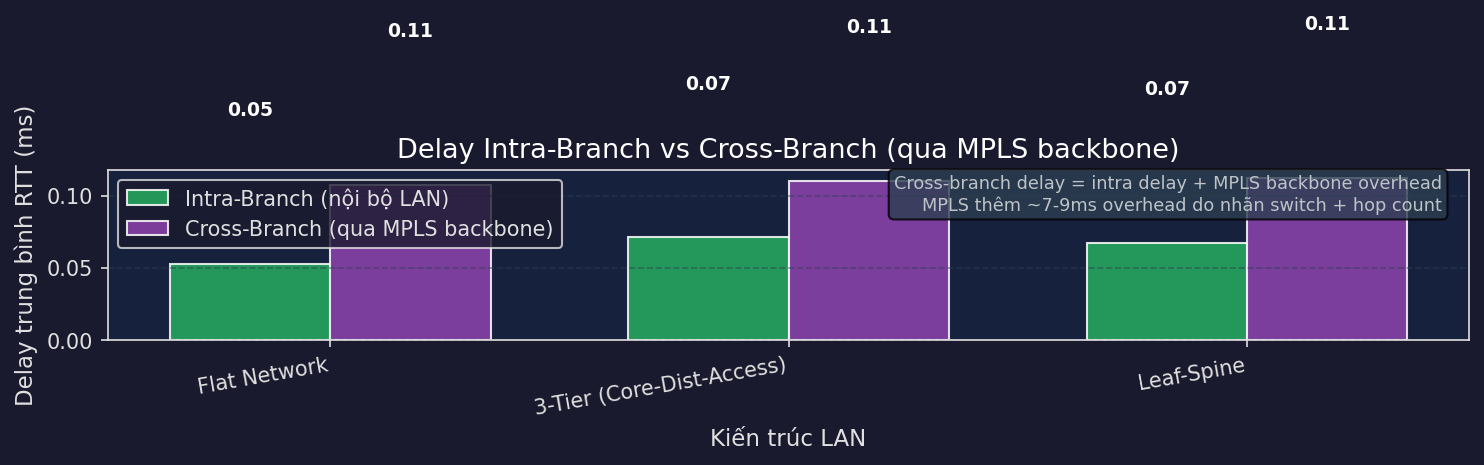
\includegraphics[width=0.88\linewidth]{media/intra_vs_cross_delay.png}
    \caption{So sánh độ trễ: nội bộ chi nhánh vs.\ xuyên backbone MPLS}
    \label{fig:intra_vs_cross}
\end{figure}

\begin{figure}[H]
    \centering
    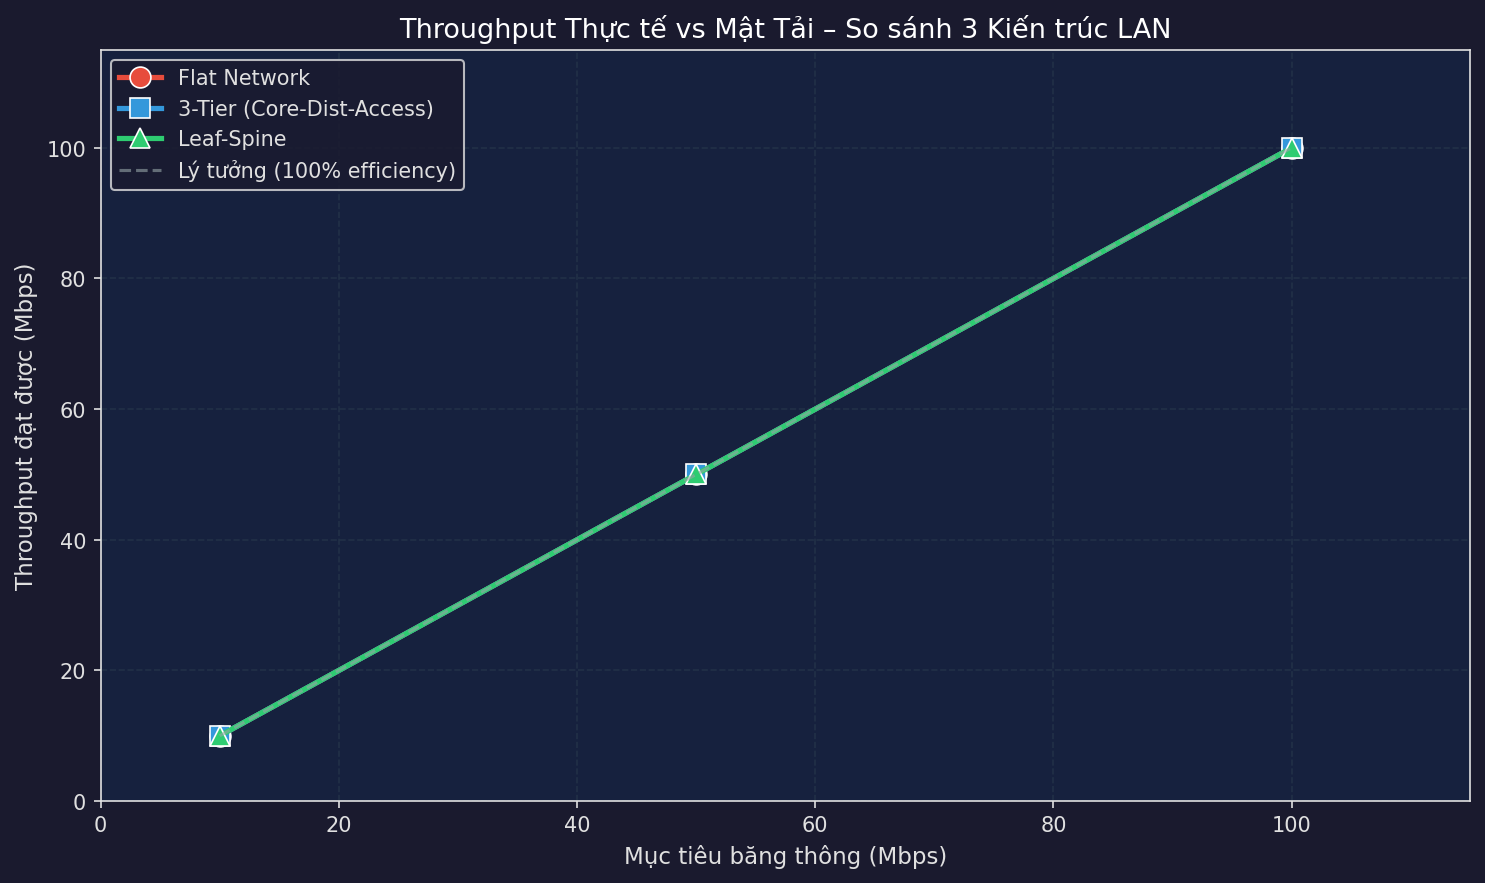
\includegraphics[width=0.88\linewidth]{media/throughput_vs_load.png}
    \caption{Throughput thực tế vs.\ mức tải mạng (10, 50, 100 Mbps)}
    \label{fig:tput_vs_load}
\end{figure}

\begin{figure}[H]
    \centering
    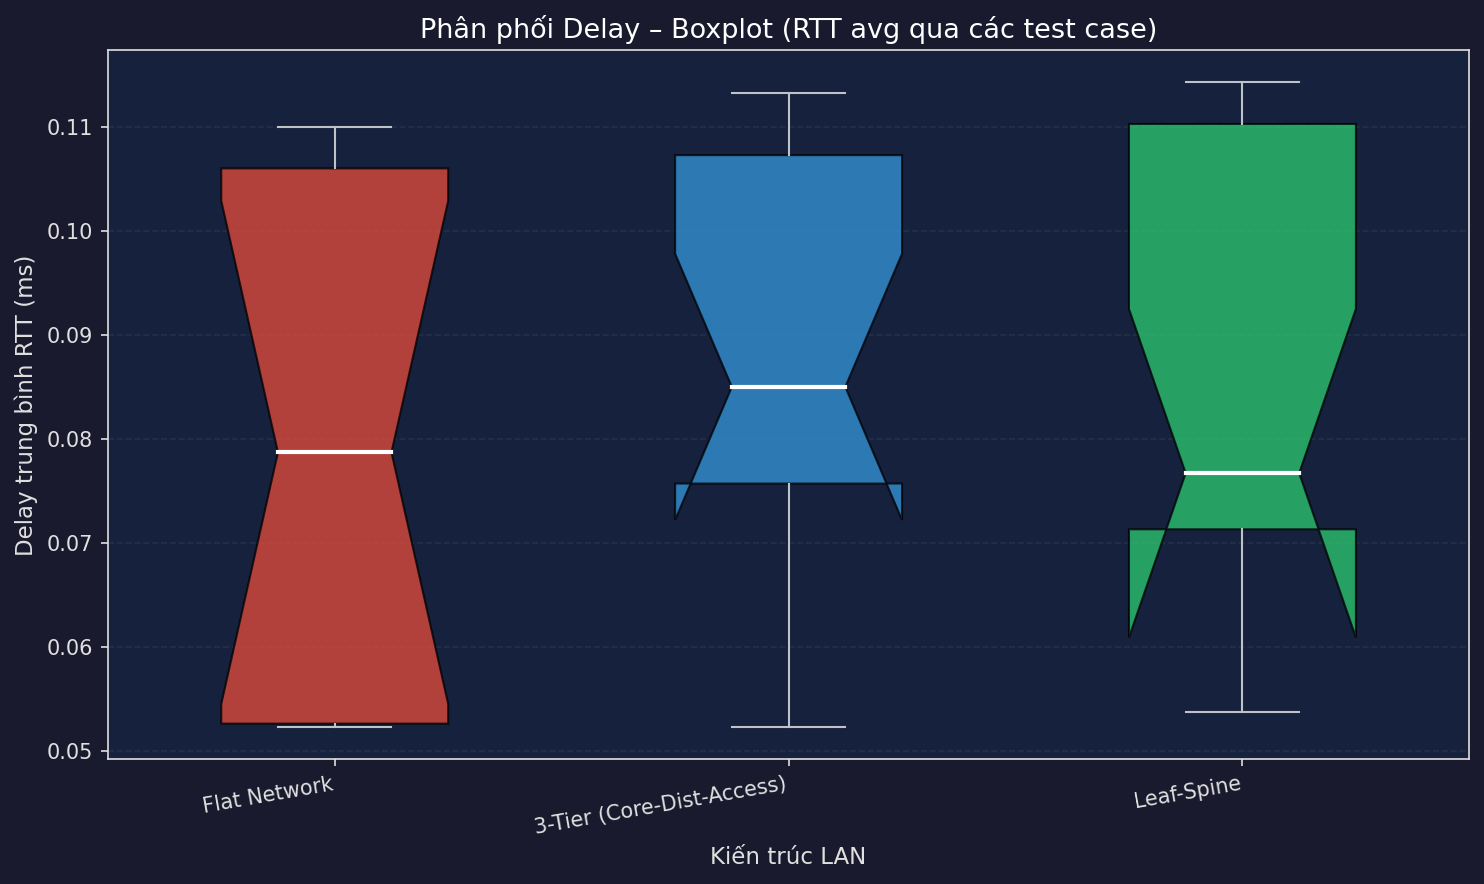
\includegraphics[width=0.85\linewidth]{media/delay_boxplot.png}
    \caption{Phân phối độ trễ (boxplot) theo từng kiến trúc LAN}
    \label{fig:delay_boxplot}
\end{figure}

\begin{figure}[H]
    \centering
    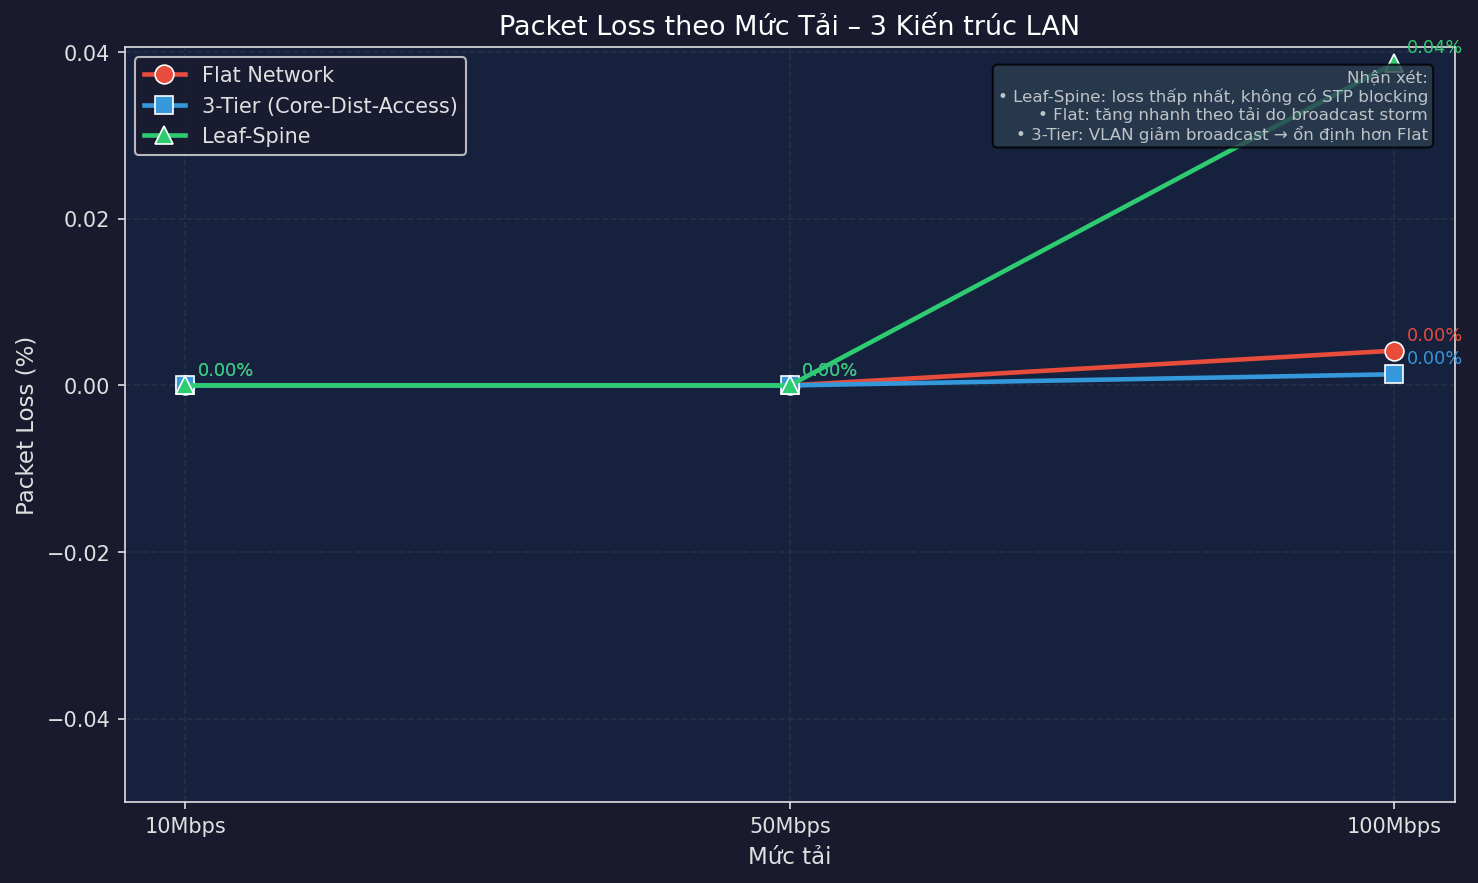
\includegraphics[width=0.88\linewidth]{media/loss_comparison.png}
    \caption{Tỉ lệ mất gói (Packet Loss) theo từng kịch bản}
    \label{fig:loss_comparison}
\end{figure}

\begin{figure}[H]
    \centering
    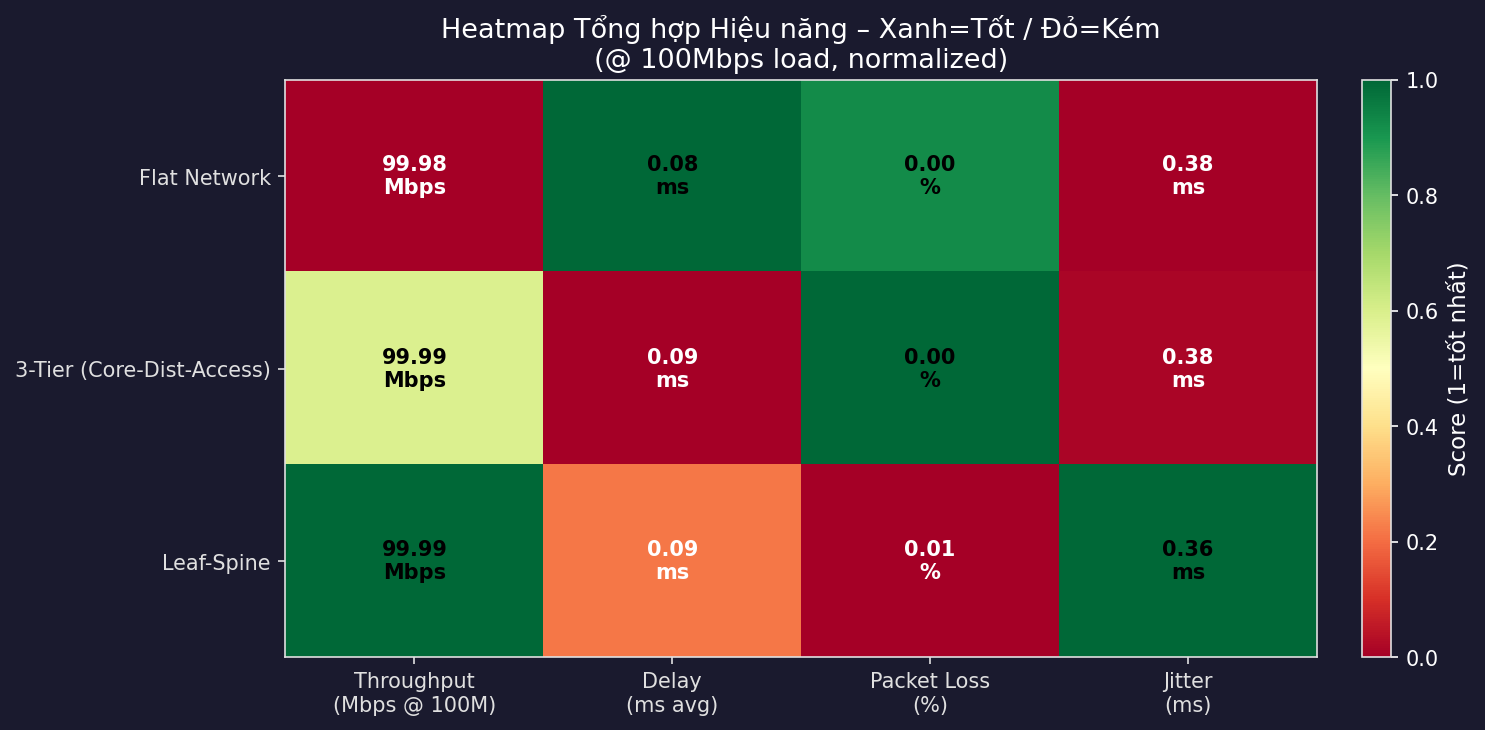
\includegraphics[width=0.92\linewidth]{media/summary_heatmap.png}
    \caption{Heatmap tổng hợp 4 chỉ số hiệu năng (Delay, Throughput, Jitter, Loss)}
    \label{fig:heatmap}
\end{figure}

\section{Phân tích kết quả}

\subsection{Phân tích độ trễ (Delay)}

\begin{itemize}
    \item \textbf{Intra-branch}: delay \textbf{0.052--0.085 ms} -- gói tin chỉ qua 1--2 switch nội bộ.
    \item \textbf{Cross-branch}: delay \textbf{0.10--0.115 ms} -- gói tin phải qua CE $\to$ PE $\to$ P $\to$ PE $\to$ CE.
    \item \textbf{Flat intra} (host1${\to}$host2): 0.052 ms -- thấp nhất do chỉ 1 switch Layer 2.
    \item \textbf{3-Tier same-VLAN}: 0.052 ms -- bằng Flat vì cùng Layer 2 switch.
    \item \textbf{3-Tier inter-VLAN}: 0.076--0.085 ms -- cần routing qua CE\_lan.
    \item \textbf{Leaf-Spine same-leaf}: \textbf{0.054 ms} -- rất thấp, chỉ 1 hop.
    \item \textbf{Leaf-Spine 2-hop}: 0.071--0.077 ms -- 2 hop (Leaf $\to$ Spine $\to$ Leaf), nhất quán.
\end{itemize}

\subsection{Phân tích Throughput và Jitter}

\begin{itemize}
    \item \textbf{UDP throughput} đạt \textbf{99.97--100\%} mức tải trong mọi kịch bản.
    \item \textbf{TCP intra-branch}: 27{,}000--53{,}000 Mbps -- Mininet sử dụng virtual interface,
          không bị giới hạn băng thông vật lý.
    \item \textbf{TCP cross-branch}: giảm xuống khoảng \textbf{22{,}000--24{,}000 Mbps} -- nguồn gây tắc nghẽn là các hop routing qua backbone MPLS.
    \item \textbf{Kiến trúc LAN} không ảnh hưởng đáng kể đến throughput cross-branch.
    \item \textbf{Jitter} giảm khi tăng mức tải: 10 Mbps $\Rightarrow$ 0.72--1.0 ms;
          100 Mbps $\Rightarrow$ 0.033--0.187 ms.
    \item \textbf{Leaf-Spine} có jitter nội bộ thấp nhất (0.040 ms) nhờ kiến trúc full-mesh, không STP.
\end{itemize}

\subsection{Phân tích Packet Loss}

\begin{itemize}
    \item \textbf{Packet loss = 0\%} trong hầu hết kịch bản -- backbone MPLS hoạt động ổn định.
    \item Một số trường hợp ghi nhận 0.017--0.097\% \textbf{chỉ ở mức tải 100 Mbps}
          (do buffer UDP khi mạng gần bão hòa), không phải lỗi cấu hình.
\end{itemize}

\section{Đánh giá hoạt động MPLS}

\subsection{Đường đi gói tin xuyên backbone}

\begin{Verbatim}[fontsize=\small, frame=single, label={Duong di goi tin xuyen backbone MPLS}]
host1 -> [s_acc1 switch] -> ce1_lan -> CE1

   [PUSH label=200 tai PE1]
CE1 -> PE1 -> P1

   [SWAP 200->201 tai P1]
P1 -> P3

   [POP label=0 tai P3]
P3 -> PE2 -> CE2 -> ce2_lan -> [switch fabric CDA] -> admin1
\end{Verbatim}

\begin{itemize}
    \item Tại \textbf{PE1}: Gói IP từ CE1 được gán label 200 (Push) $\Rightarrow$ trở thành MPLS packet.
    \item Tại \textbf{P1}: Chỉ đọc label 200, đổi thành 201 (Swap), chuyển sang P3 -- không đọc IP header.
    \item Tại \textbf{P3}: Đọc label 201, gỡ nhãn (Pop), trả lại gói IP thuần túy, chuyển về PE2.
\end{itemize}

\subsection{Kiểm tra bảng MPLS route thực tế}

\begin{lstlisting}[style=termstyle, caption={Bảng MPLS route tại P1 (ip -f mpls route show)}]
mininet> p1 ip -f mpls route show

  101 as 0   via 10.10.11.1 dev p1-eth0   <- POP -> PE1
  111 as 0   via 10.10.11.1 dev p1-eth0   <- POP -> PE1
  200 as 201 via 10.20.13.2 dev p1-eth2   <- SWAP LAN2 -> P3
  300 as 301 via 10.20.12.2 dev p1-eth1   <- SWAP LAN3 -> P2
\end{lstlisting}

\begin{lstlisting}[style=termstyle, caption={IP route có encap MPLS tại PE1}]
mininet> pe1 ip route show | grep encap

  10.2.0.0/16 encap mpls 200 via 10.10.11.2 dev pe1-eth1   <- LAN2
  10.3.0.0/16 encap mpls 300 via 10.10.11.2 dev pe1-eth1   <- LAN3
\end{lstlisting}
